\documentclass[10pt]{article}
\usepackage[margin=1in]{geometry}
\usepackage{amsmath, amssymb, cancel, xcolor, mathtools, graphicx}
\graphicspath{ {./images/} }

\newcommand\hcancel[2][black]{\setbox0=\hbox{$#2$}%
\rlap{\raisebox{.45\ht0}{\textcolor{#1}{\rule{\wd0}{1pt}}}}#2} 

\begin{document}

\begin{flushleft}
    Brandon Szeto \\
    Professor Kenneth Zeger \\
	ECE 109 \\
\end{flushleft}

\begin{center}
	\Large \textbf{Week 4, Lecture 01-31-23}
\end{center}
\normalsize

\begin{flushleft}

\begin{itemize}
    \item[\textbf{\underline{Example:}}] \textbf{Given the sample space:}
        $$ S = \{H, TH, TTH, TTTH, ... \} $$
        Flip a fair coin until 1st head appears, then stop. 
        Let us define the random variable $X = $ number of tosses until 1st head:
        $$ \begin{aligned}
            X(H) &= 1 \\
            X(TH) &= 2 \\
            X(TTH) &= 3 \\
            \vdotswithin{} \\
            P(X = 1) &= P(H) = \frac{1}{2} \\
            P(X = 2) &= P(TH) = \frac{1}{2^2} \\
            \vdotswithin{} \\
            P(X = n) &= P(T ... TH) = \frac{1}{2^n} \\
        \end{aligned} $$
        Define a second random variable Y to indicate oddness:
        $$ \begin{aligned} Y &= 
        \begin{cases}
            1 \text{ if X is odd} \\
            0 \text{ if X is even} \\
        \end{cases}
        Y(H) &= 1 \text{     odd} \\
        Y(TH) &= 0 \text{     even} \\
        Y(TTH) &= 1 \text{     odd} \\
        Y(TTTH) &= 0 \text{     even} \\
        \vdotswithin{}
    \end{aligned}
        $$
        What is $P(Y = 0)$ ?
        $$ \begin{aligned}
            P(Y = 0) &= P(X is even) \\
                     &= P(X = 2) + P(X = 4) + P(X = 6) + ... \\
                     &= \frac{1}{2^2} + \frac{1}{2^4} \frac{1}{2^6} + ...
                     \text{ geometric series} \\
                     &= \frac{\frac{1}{4}}{1 - \frac{1}{4}} * \frac{4}{4} =
                     \frac{1}{4 - 1} = \frac{1}{3}
        \end{aligned} $$
        Consequently,
        $$ P(Y = 1) = 1 - P(Y = 0) = 1 - \frac{1}{3} = \frac{2}{3} $$
        \textbf{Note:}
            $$ \begin{aligned}
                \{ Y = 0 \} &= \{ u \in S : Y(u) = 0 \}  \\
                            &= \{ TH, TTTH, TTTTTH, ... \}
            \end{aligned} $$
\end{itemize}

\textbf{\underline{Notation:}} \\
Let $A \subseteq R $ (i.e. a set of real numbers). We will use the following
notation:

$$ \boxed{
    \{ X \in A \} = \{ u \in S : X(u) \in A \}
}$$

In the previous example we can write
$$ \begin{aligned}
    \{ Y = 0 \} &= \{ Y \in \{0\}\} \\
    \{ X \leq 4 \} &= \{ X \in (-\infty, 4]\} \\
    \{ -1 \leq X < 7 \} &= \{ X \in [-1, 7)\} \\
    \vdotswithin{}
\end{aligned} $$

\begin{itemize}
    \item[\textbf{\underline{Example:}}] \textbf{Flip biased coin 3 times. $P(H)
        = q$. Define random variable $X =$ number of heads (i.e. 0, 1, 2, 3).
    What is $P(X \leq 1)$ ?}
    $$ \{ X \leq 1 \} \text{ is the event } \{ TTT, HTT, THT, TTH \} $$
    $$ \begin{aligned}
        P(X \leq 1) &= P( \{ TTT, HTT, THT, TTH \} ) \\
                    &= (1 - q)^3 + 3q(1 - q)^2
    \end{aligned} $$
\end{itemize}

\begin{center}
    \noindent\rule{6.5in}{0.4pt}
\end{center}

\textbf{Fundamental question about a random variable $X$ is this:}
$$ \text{What is } P(X \leq \text{something}) ?$$
Recall the CDF (Cummulative Distribution Function) of random variable $X$ :
$$ F_x(u) = P(X \leq u) \text{ for } -\infty < u < \infty$$
\begin{itemize}
    \item Always use uppercase $F$ for CDF.
    \item The $X$ indicates which random variable
    \item Try not to use $X$ as the argument. Any other variable is ok. e.g. u,
        v, w, a, b, c
\end{itemize}

\begin{itemize}
    \item[\textbf{\underline{Example:}}] \textbf{Flip a fair coin 2 times.}
        $$ S = \{HH, HT, TH, TT\} $$
        Define random variable $X = $ number of heads $\in \{0, 1, 2\}$. Find
        CDF of $X$.
        $$ \begin{aligned}
            P(X = 0) &= P(TT) = \frac{1}{4} \\
            P(X = 1) &= P(HT \text{ or } TH) = \frac{1}{2} \\
            P(X = 2) &= P(HH) = \frac{1}{4} \\
        \end{aligned} $$

        \begin{center}
            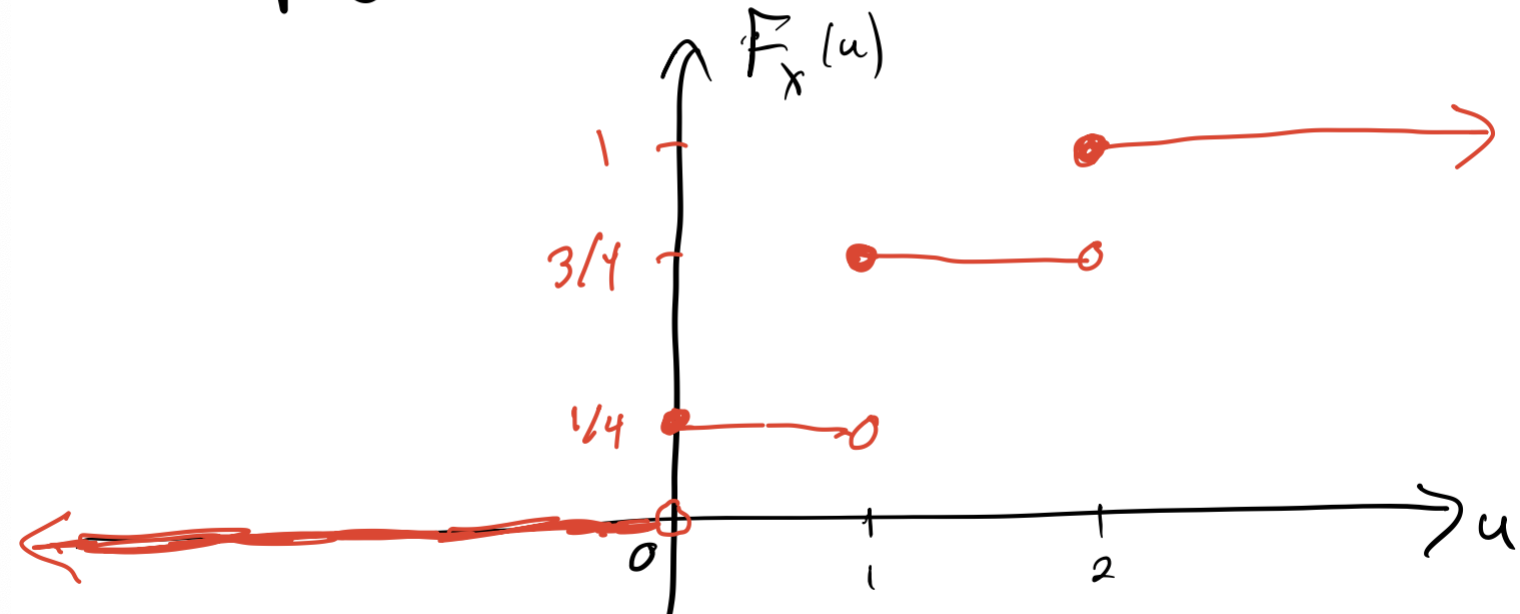
\includegraphics[width=6in, height=2in]{Week_4.1}
        \end{center}

        \underline{Cases:}
        $$ \begin{aligned}
            u < 0 &=> P(X \leq u) = 0 \\
            u = 0 &=> P(X \leq u) = P(X \leq 0) = P(X = 0) = \frac{1}{4} \\
            0 \leq u < 1 &=> P(X \leq u) = P(X = 0) = \frac{1}{4} \\
            1 \leq u < 2 &=> P(X \leq u) = P(X = 0 \text{ or } X = 1) =
            \frac{1}{4} + \frac{1}{2} = \frac{3}{4} \\
            u \geq 2 &=> P(X \leq u) = 1
        \end{aligned} $$
    \item[\textbf{\underline{Example:}}] \textbf{Suppose an experiment has
        sample space}
        $$ S = [0, 1] $$
        Suppose $P([a,b]) = b - a$ whenever $0 \leq a \leq b \leq 1$

        \begin{center}
            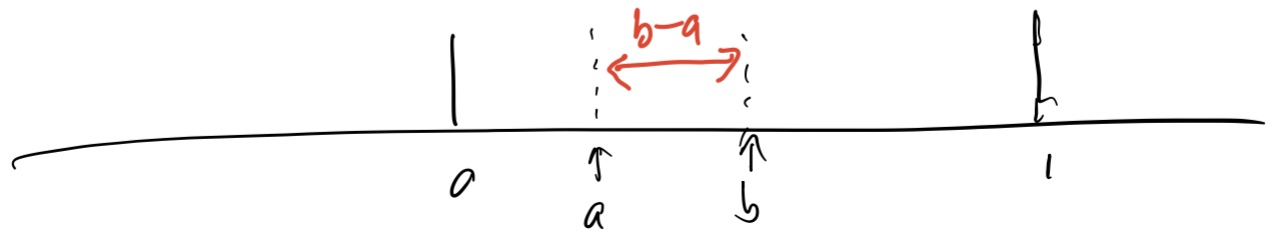
\includegraphics[width=6in, height=1in]{Week_4.2}
        \end{center}

        Define a random variable $X$ as in the following diagram:

        \begin{center}
            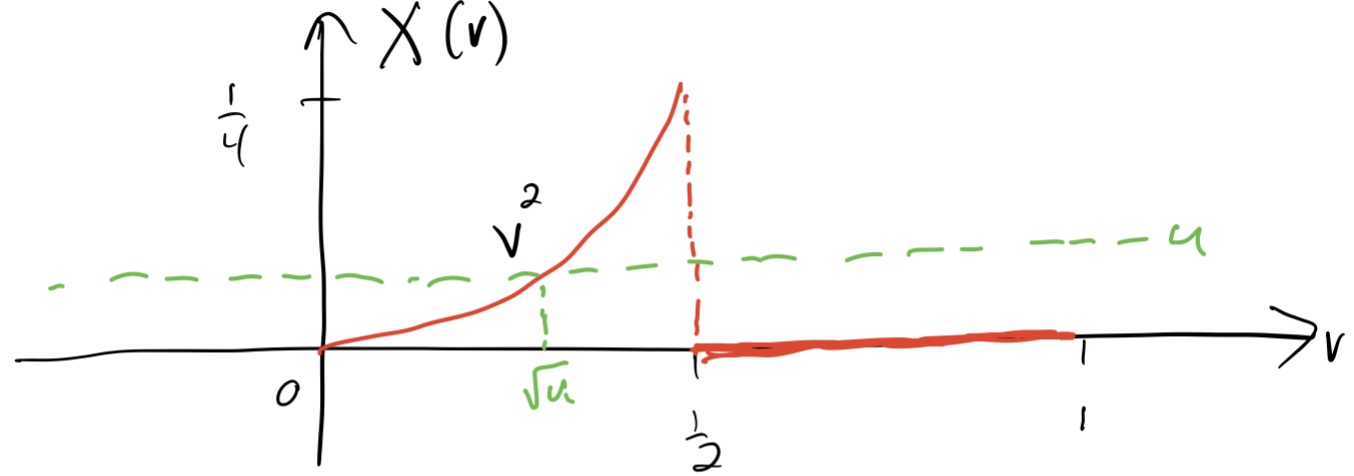
\includegraphics[width=6in, height=2in]{Week_4.3}
        \end{center}

        What is the CDF of $X$? Need to compute $P(X \leq u)$ for all $u$.

        \begin{center}
            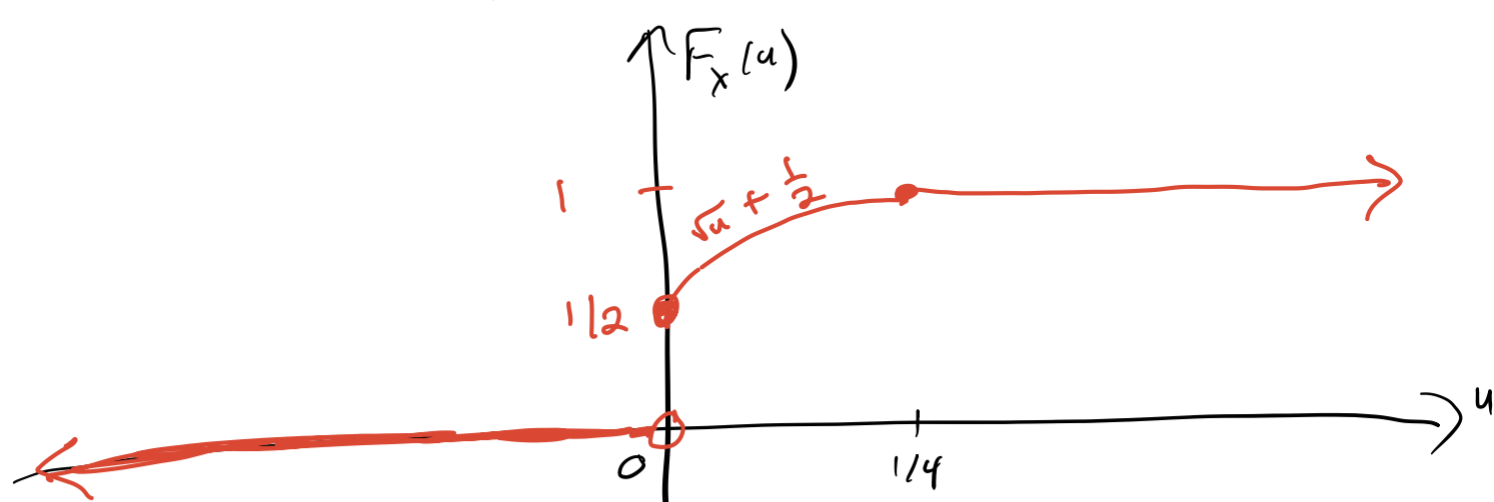
\includegraphics[width=6in, height=2in]{Week_4.4}
        \end{center}

        \underline{Cases:}
        $$ \begin{aligned}
            u < 0 &: \text{It's never true that } X \leq u. \text{ So } F_x(u) = P(X
                \leq u) = 0 \\
            u = 0 &: P(X \leq 0) = P(X = 0) = P(\{ 0 \} \cup [ \frac{1}{2}, 1])
                \\
                  &= P(\{ 0 \}) + P( [ \frac{1}{2}, 1] ) \\
                  &= P(\{ [ 0, 0 ] \}) + P( [ \frac{1}{2}, 1] ) \\
                  &= 0 + \frac{1}{2} = \frac{1}{2} \\
            u \geq \frac{1}{4} &: P(X \leq u) = P([0,1]) = 1 \\
            0 \leq u < \frac{1}{4} &: P(X \leq u) = P([0, \sqrt{u}] \cup
            [\frac{1}{2}, 1]) \\
                                   &= \sqrt{u} + \frac{1}{2}
        \end{aligned} $$
\end{itemize}

\textbf{Some properties of CDFs:}
\begin{enumerate}
    \item $0 \leq F_x(u) \leq 1$
    \item If $a < b$, then $F(a) \leq F(b)$. Since $P(X \leq b) = P(X \leq a) +
        P(a < X \leq b)$ 
    \item $F(\infty) = \lim_{u \to \infty} F(u) = 1$
    \item $F(-\infty) = \lim_{u \to -\infty} F(u) = 0$
    \item F(u) is right-continuous. If you approach $u$ from the right, it's
        continuous, but not necessarily from the left.
\end{enumerate}

\textbf{Some computation facts:}

     $$ \begin{aligned}
            P(X > u) &= P(\{X \leq u\}^c) \\
            &= 1 - P(X \leq u) \\
            &= 1 - F(u) \\
            P(X < u) &= P(X \leq u) - P(X = u) \\
            &= F(u^-) \\
            P(X = u) &= 1 - P(X < u) = 1 - F(u^-) \\
            P(X = u) &= P(X \leq u) - P(X < u) \\
            &= F(u) - F(u^-) \\
            P(a < X \leq b) &= P(X \leq b) - P(X \leq a) \\
            &= F(b) - F(a) \\
            P(a < X < b) &= F(b^-) - F(a) \\
            P(a \leq X < b) &= F(b^-) - F(a^-) \\
            P(a < X \leq b) &= F(b^-) - F(a^-) \\
        \end{aligned} $$

If $F(u)$ is continuous at $u = a$, then there is no jump at a. Thus, $P(a < X
\leq b) = P(a \leq X \leq b)$ since $F(a) = F(a^+) = F(a^-)$. 
$$\therefore P(X = a) = 0$$

\end{flushleft}

\end{document}
